%!TeX encoding = UTF-8
\documentclass[notheorems, aspectratio=54]{beamer}
% aspectratio: 1610, 149, 54, 43(default), 32
\usepackage[utf8]{inputenc}
\usepackage[vietnamese]{babel}
\usepackage{latexsym}
\usepackage{amsmath,amssymb}
\usepackage{mathtools}
\usepackage{color,xcolor}
\usepackage{graphicx}
\usepackage{algorithm}
\usepackage{amsthm}
\usepackage{lmodern} % 解决 font warning
% \usepackage[UTF8]{ctex}
\usepackage{animate} % insert gif

\usepackage{lipsum} % To generate test text 
\usepackage{ulem} % 下划线,波浪线

\usepackage{listings} % display code on slides; don't forget [fragile] option after \begin{frame}

% ----------------------------------------------
% tikx
\usepackage{framed}
\usepackage{tikz}
\usepackage{pgf}
\usetikzlibrary{calc,trees,positioning,arrows,chains,shapes.geometric,%
	decorations.pathreplacing,decorations.pathmorphing,shapes,%
	matrix,shapes.symbols}
\pgfmathsetseed{1} % To have predictable results
% Define a background layer, in which the parchment shape is drawn
\pgfdeclarelayer{background}
\pgfsetlayers{background,main}

% define styles for the normal border and the torn border
\tikzset{
	normal border/.style={orange!30!black!10, decorate, 
		decoration={random steps, segment length=2.5cm, amplitude=.7mm}},
	torn border/.style={orange!30!black!5, decorate, 
		decoration={random steps, segment length=.5cm, amplitude=1.7mm}}}

% Macro to draw the shape behind the text, when it fits completly in the
% page
\def\parchmentframe#1{
	\tikz{
		\node[inner sep=2em] (A) {#1};  % Draw the text of the node
		\begin{pgfonlayer}{background}  % Draw the shape behind
			\fill[normal border] 
			(A.south east) -- (A.south west) -- 
			(A.north west) -- (A.north east) -- cycle;
\end{pgfonlayer}}}

% Macro to draw the shape, when the text will continue in next page
\def\parchmentframetop#1{
	\tikz{
		\node[inner sep=2em] (A) {#1};    % Draw the text of the node
		\begin{pgfonlayer}{background}    
			\fill[normal border]              % Draw the ``complete shape'' behind
			(A.south east) -- (A.south west) -- 
			(A.north west) -- (A.north east) -- cycle;
			\fill[torn border]                % Add the torn lower border
			($(A.south east)-(0,.2)$) -- ($(A.south west)-(0,.2)$) -- 
			($(A.south west)+(0,.2)$) -- ($(A.south east)+(0,.2)$) -- cycle;
\end{pgfonlayer}}}

% Macro to draw the shape, when the text continues from previous page
\def\parchmentframebottom#1{
	\tikz{
		\node[inner sep=2em] (A) {#1};   % Draw the text of the node
		\begin{pgfonlayer}{background}   
			\fill[normal border]             % Draw the ``complete shape'' behind
			(A.south east) -- (A.south west) -- 
			(A.north west) -- (A.north east) -- cycle;
			\fill[torn border]               % Add the torn upper border
			($(A.north east)-(0,.2)$) -- ($(A.north west)-(0,.2)$) -- 
			($(A.north west)+(0,.2)$) -- ($(A.north east)+(0,.2)$) -- cycle;
\end{pgfonlayer}}}

% Macro to draw the shape, when both the text continues from previous page
% and it will continue in next page
\def\parchmentframemiddle#1{
	\tikz{
		\node[inner sep=2em] (A) {#1};   % Draw the text of the node
		\begin{pgfonlayer}{background}   
			\fill[normal border]             % Draw the ``complete shape'' behind
			(A.south east) -- (A.south west) -- 
			(A.north west) -- (A.north east) -- cycle;
			\fill[torn border]               % Add the torn lower border
			($(A.south east)-(0,.2)$) -- ($(A.south west)-(0,.2)$) -- 
			($(A.south west)+(0,.2)$) -- ($(A.south east)+(0,.2)$) -- cycle;
			\fill[torn border]               % Add the torn upper border
			($(A.north east)-(0,.2)$) -- ($(A.north west)-(0,.2)$) -- 
			($(A.north west)+(0,.2)$) -- ($(A.north east)+(0,.2)$) -- cycle;
\end{pgfonlayer}}}

% Define the environment which puts the frame
% In this case, the environment also accepts an argument with an optional
% title (which defaults to ``Example'', which is typeset in a box overlaid
% on the top border
\newenvironment{parchment}[1][Example]{%
	\def\FrameCommand{\parchmentframe}%
	\def\FirstFrameCommand{\parchmentframetop}%
	\def\LastFrameCommand{\parchmentframebottom}%
	\def\MidFrameCommand{\parchmentframemiddle}%
	\vskip\baselineskip
	\MakeFramed {\FrameRestore}
	\noindent\tikz\node[inner sep=1ex, draw=black!20,fill=white, 
	anchor=west, overlay] at (0em, 2em) {\sffamily#1};\par}%
{\endMakeFramed}

% ----------------------------------------------

\mode<presentation>{
	\usetheme{CambridgeUS}
	% Boadilla CambridgeUS
	% default Antibes Berlin Copenhagen
	% Madrid Montpelier Ilmenau Malmoe
	% Berkeley Singapore Warsaw
	\usecolortheme{beaver}
	% beetle, beaver, orchid, whale, dolphin
	\useoutertheme{infolines}
	% infolines miniframes shadow sidebar smoothbars smoothtree split tree
	\useinnertheme{circles}
	% circles, rectanges, rounded, inmargin
}
% 设置 block 颜色
\setbeamercolor{block title}{bg=red!30,fg=white}

\newcommand{\reditem}[1]{\setbeamercolor{item}{fg=red}\item #1}

% 缩放公式大小
\newcommand*{\Scale}[2][4]{\scalebox{#1}{\ensuremath{#2}}}

% 解决 font warning
\renewcommand\textbullet{\ensuremath{\bullet}}

% ---------------------------------------------------------------------
% flow chart
\tikzset{
	>=stealth',
	punktchain/.style={
		rectangle, 
		rounded corners, 
		% fill=black!10,
		draw=white, very thick,
		text width=6em,
		minimum height=2em, 
		text centered, 
		on chain
	},
	largepunktchain/.style={
		rectangle,
		rounded corners,
		draw=white, very thick,
		text width=10em,
		minimum height=2em,
		on chain
	},
	line/.style={draw, thick, <-},
	element/.style={
		tape,
		top color=white,
		bottom color=blue!50!black!60!,
		minimum width=6em,
		draw=blue!40!black!90, very thick,
		text width=6em, 
		minimum height=2em, 
		text centered, 
		on chain
	},
	every join/.style={->, thick,shorten >=1pt},
	decoration={brace},
	tuborg/.style={decorate},
	tubnode/.style={midway, right=2pt},
	font={\fontsize{10pt}{12}\selectfont},
}
% ---------------------------------------------------------------------

% code setting
\lstset{
	language=C++,
	basicstyle=\ttfamily\footnotesize,
	keywordstyle=\color{red},
	breaklines=true,
	xleftmargin=2em,
	numbers=left,
	numberstyle=\color[RGB]{222,155,81},
	frame=leftline,
	tabsize=4,
	breakatwhitespace=false,
	showspaces=false,               
	showstringspaces=false,
	showtabs=false,
	morekeywords={Str, Num, List},
}

\setbeamerfont{bibliography item}{size=\footnotesize}
\setbeamerfont{bibliography entry author}{size=\footnotesize}
\setbeamerfont{bibliography entry title}{size=\footnotesize}
\setbeamerfont{bibliography entry location}{size=\footnotesize}
\setbeamerfont{bibliography entry note}{size=\footnotesize}
% ---------------------------------------------------------------------

%% preamble
\title[Know \& Share Week 1]{GIỚI THIỆU TỔNG QUAN VỀ ĐỒ THỊ TRI THỨC}
% \subtitle{The subtitle}
\author{Lê Nhựt Nam KHMT-K18}
\institute[HCMUS]{Đại học Khoa học Tự nhiên, Đại học Quốc gia TP Hồ Chí Minh}

% -------------------------------------------------------------

\begin{document}
	
	%% title frame
	\begin{frame}
		\titlepage
	\end{frame}

	\begin{frame}{Nội dung trình bày}
		\tableofcontents
	\end{frame}
	%% normal frame
	\section{Đồ thị tri thức}
	\begin{frame}{Đồ thị}
		\begin{figure}[H]
			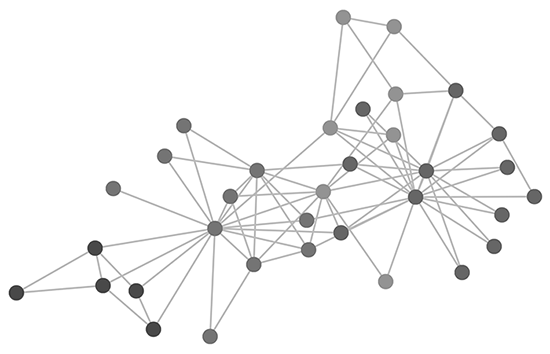
\includegraphics[width=0.9\linewidth]{figs/graph.png}
			\caption{Ví dụ minh họa một đồ thị}
			\label{fig:writing-thesis}
		\end{figure}
	\end{frame}
	\begin{frame}{Tri thức là gì}
		\begin{figure}[H]
			
\includegraphics[width=1\linewidth]{figs/knowledge.png}
		\end{figure}
	\end{frame}
	\begin{frame}{Lịch sử của Đồ thị tri thức}
		\begin{figure}[H]
			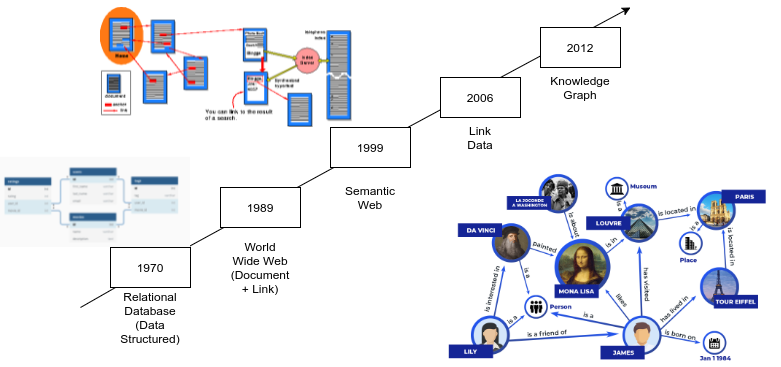
\includegraphics[width=1\linewidth]{figs/history_kg.png}
			\caption{Lịch sử của đồ thị tri thức}
			\label{fig:writing-thesis}
		\end{figure}
	\end{frame}
	\begin{frame}{Ví dụ về Đồ thị tri thức}
		\begin{figure}[H]
			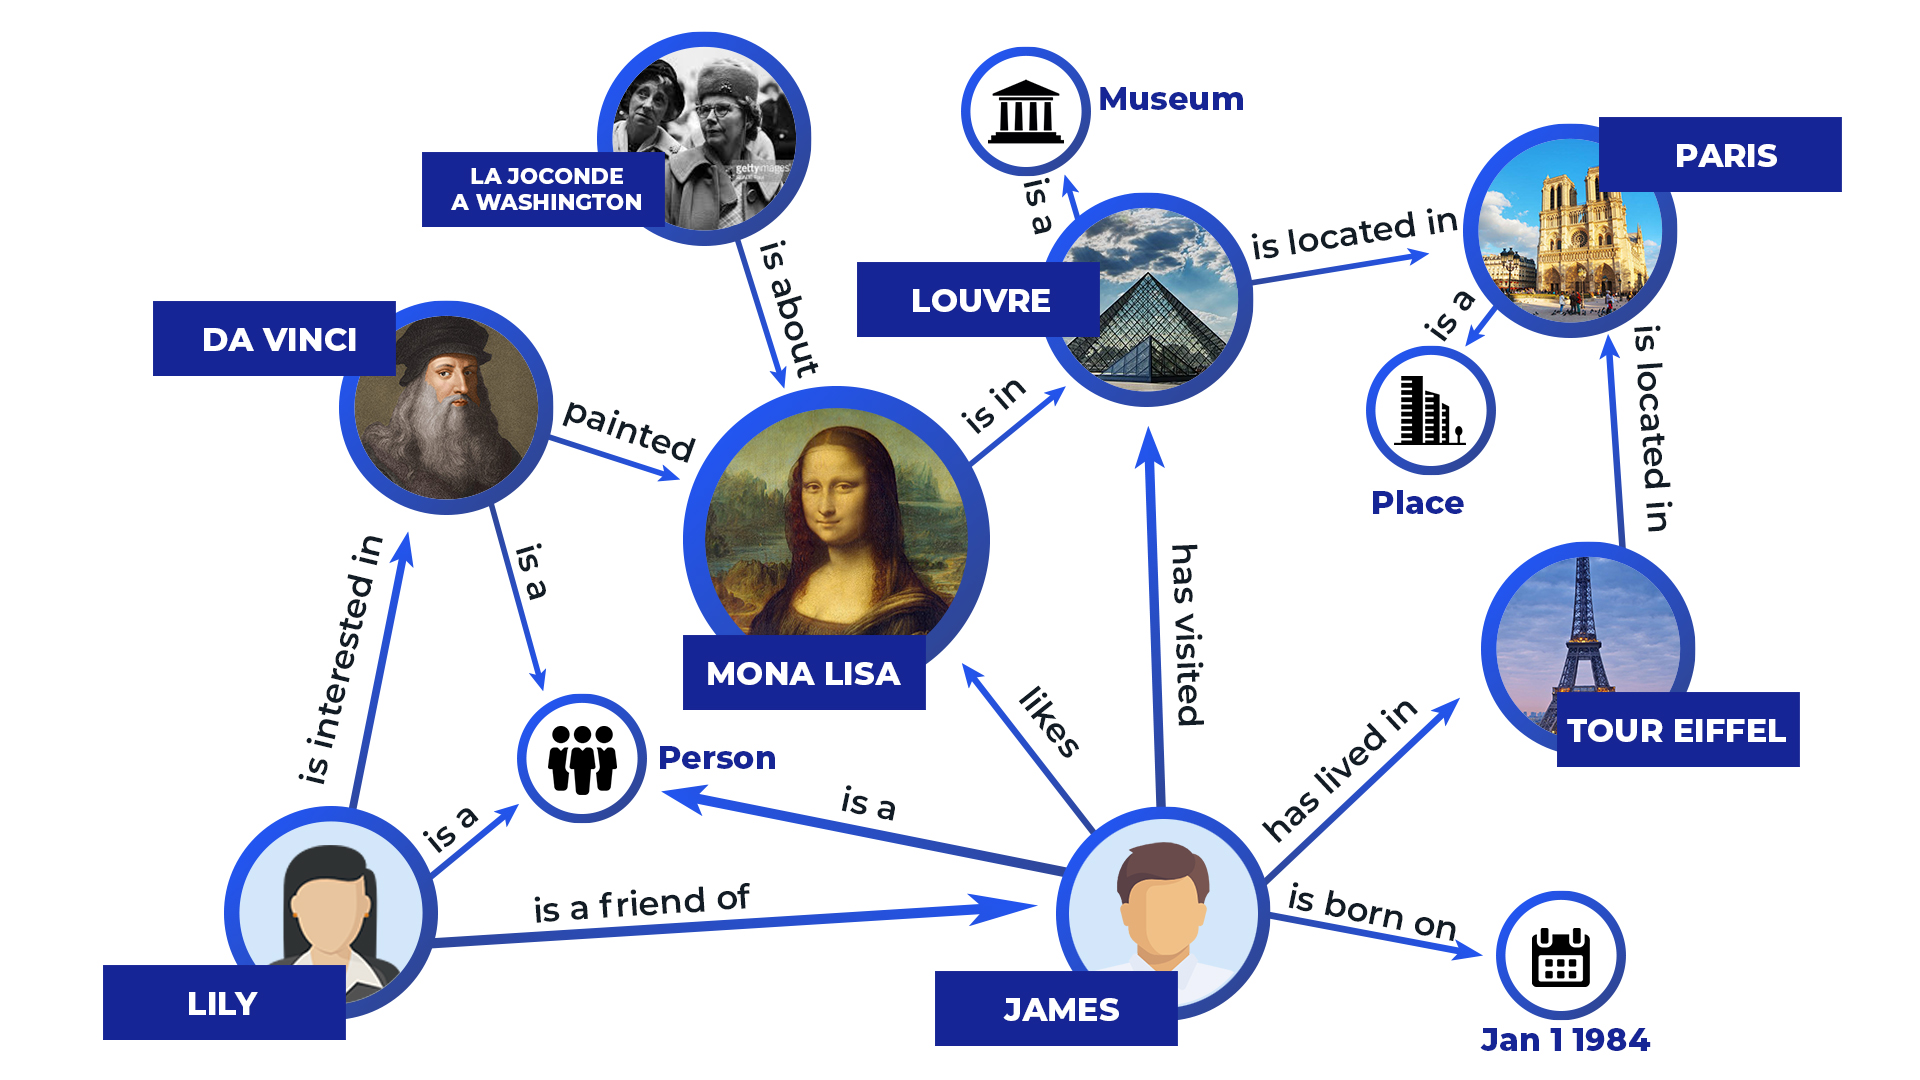
\includegraphics[width=1\linewidth]{figs/knowledge-graph.jpg}
			\caption{Ví dụ về đồ thị tri thức}
			\label{fig:writing-thesis}
		\end{figure}
	%Include: entities, attributes, relationships
	
	%Nodes are entities
	
	%Nodes have attribute tags (can contain types)
	
	%The edges of two nodes are the relationship between entities
	\end{frame}
	\begin{frame}{Knowledge Graph vs Deep Learning}
		\begin{block}{~\vspace{0.7cm}}
			\begin{center}
				\vspace{-0.8cm}
				\begin{tabular}{p{0.45\textwidth}|p{0.45\textwidth}}
					\textcolor{white}{\bf Knowledge Graph} & \textcolor{white}{\bf Deep Learning} \\\\
					Suy nghĩ & Não bộ\\
					Tìm kiếm, tương tác người máy & Trí tuệ tri giác, nhiều loại tác vụ về dáng, giọng nói, hình ảnh, video\\
					Trí thức lớn, giải thích được, hiểu được & Dữ liệu huấn luyện lớn, sức mạnh tính toán, khó giải thích\\
					Mạnh về trí thức, yếu suy luận & Mạnh hơn con người ở nhiều tác vụ\\
				\end{tabular}
			\end{center}
		\end{block}
	Xu hướng: Kết hợp Knowledge Graph và Deep Learning
	\end{frame}

	\begin{frame}{Knowledge Graph vs. Traditional Knowledge Base vs. Database}
		\begin{table}[htbp]
			\caption{Bảng so sánh}\label{tab1}
			\resizebox{\columnwidth}{!}{\begin{tabular}{|l|l|l|l|}
					\hline
					 &  Semantic layer &Data layer & \\
					\hline
					Relational database & Không có ngữ nghĩa & Giàu dữ liệu & Thành công\\
					Traditional knowledge base &Giàu ngữ nghĩa & Có ít thể hiện & \\
					Knowledge Graph & Một lượng nhỏ ngữ nghĩa  & Giàu thể hiện & Thành công\\
					\hline
			\end{tabular}}
		\end{table}
	\end{frame}
	
	\section{Một số đồ thị tri thức kinh điển}
	\begin{frame}{Một số đồ thị tri thức kinh điển}
		\begin{columns}
			\begin{column}{0.5\textwidth}
				\begin{figure}[H]
					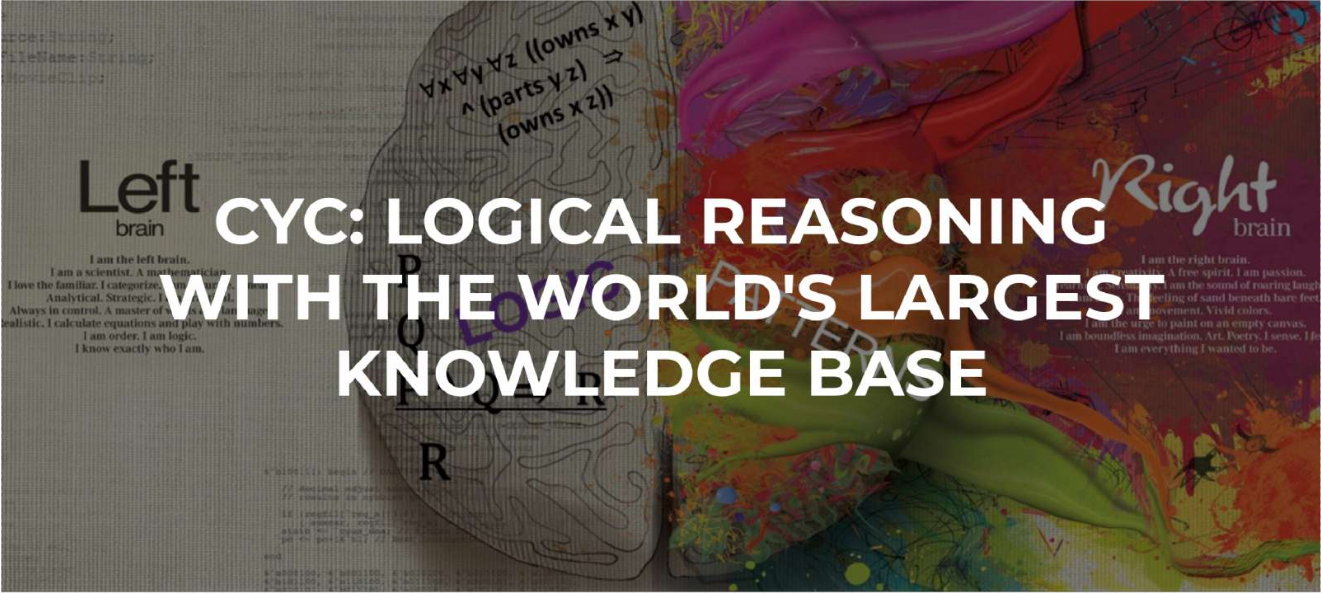
\includegraphics[width=0.5\linewidth]{figs/cyc.png}
					\label{fig:writing-thesis}
				\end{figure}
				\begin{figure}[H]
					
\includegraphics[width=0.5\linewidth]{figs/wordnet.png}
					\label{fig:writing-thesis}
				\end{figure}
				\begin{figure}[H]
					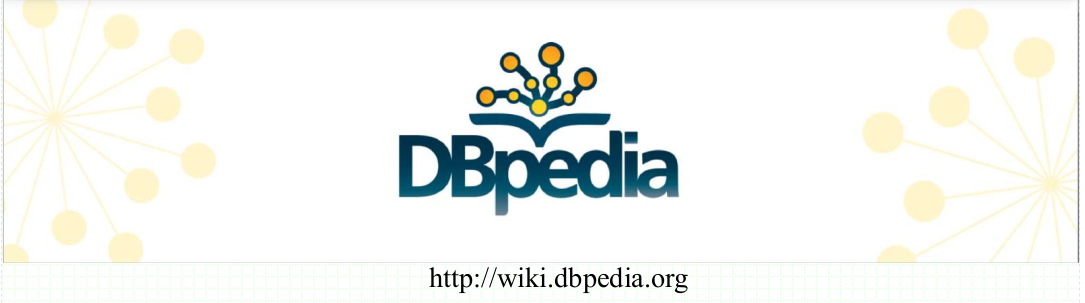
\includegraphics[width=0.5\linewidth]{figs/dbpedia.png}
					\label{fig:writing-thesis}
				\end{figure}
				\begin{figure}[H]
					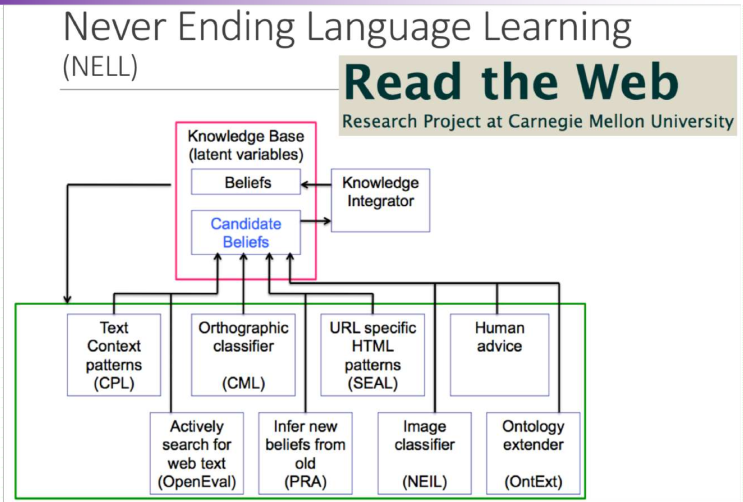
\includegraphics[width=1\linewidth]{figs/nell.png}
					\label{fig:writing-thesis}
				\end{figure}
			\end{column}
			\begin{column}{0.5\textwidth}
				\begin{figure}[H]
					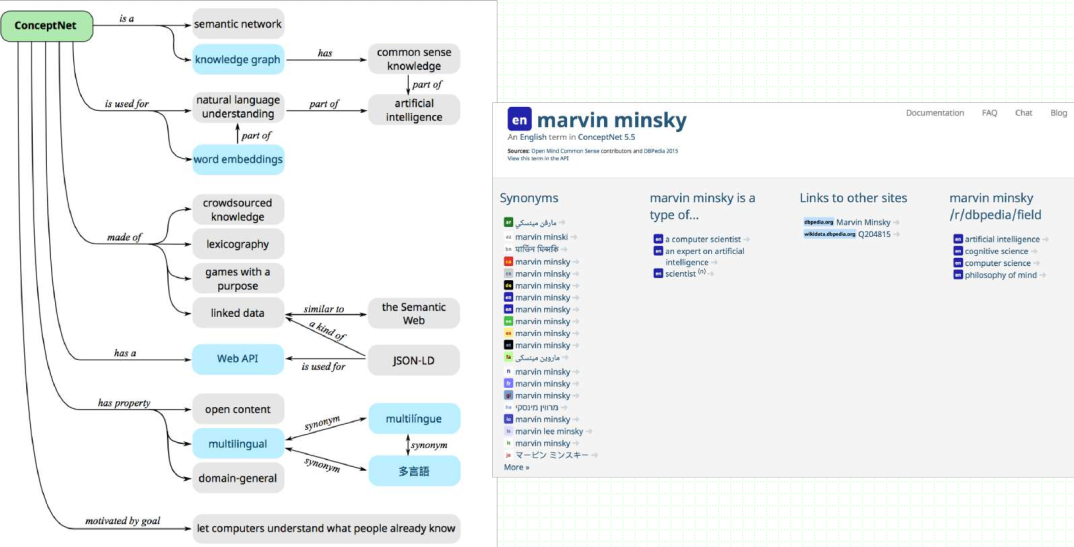
\includegraphics[width=0.5\linewidth]{figs/conceptnet.png}
					\label{fig:writing-thesis}
				\end{figure}
				\begin{figure}[H]
					
\includegraphics[width=0.5\linewidth]{figs/fb.png}
					\label{fig:writing-thesis}
				\end{figure}
				\begin{figure}[H]
					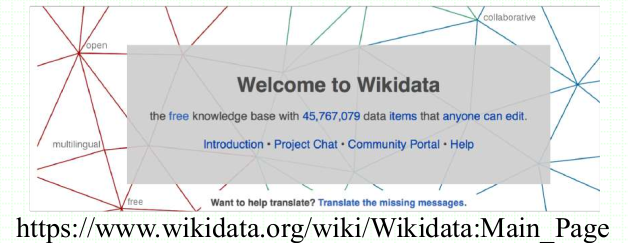
\includegraphics[width=0.5\linewidth]{figs/wikidata.png}
					\label{fig:writing-thesis}
				\end{figure}
				\begin{figure}[H]
					
\includegraphics[width=0.5\linewidth]{figs/yago.png}
					\label{fig:writing-thesis}
				\end{figure}
			\end{column}
		\end{columns}		
	\end{frame}
	\section{Một số ứng dụng của đồ thị tri thức}
	\begin{frame}{Tổ chức tri thức trên Internet}
		\begin{columns}
			\begin{column}{0.5\textwidth}
				\begin{figure}[H]
					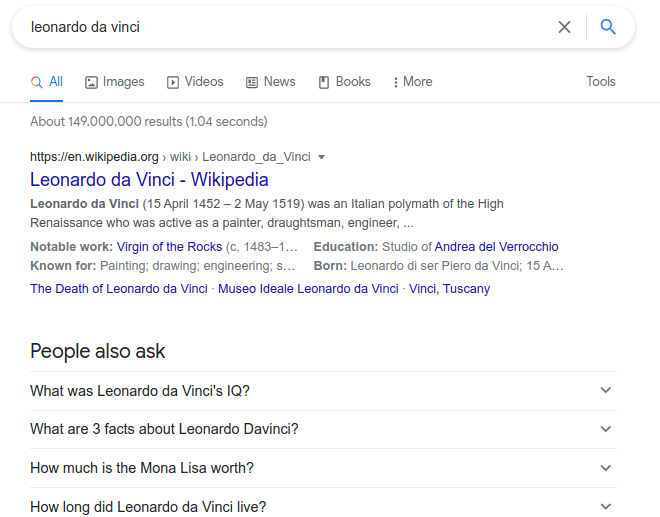
\includegraphics[width=1\linewidth]{figs/search_01.png}
				\end{figure}
			\end{column}
			\begin{column}{0.5\textwidth}
				\begin{figure}[H]
					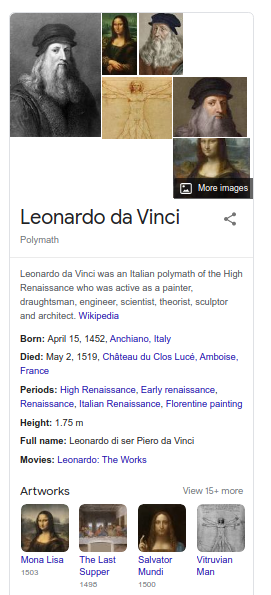
\includegraphics[width=0.5\linewidth]{figs/search_02.png}
				\end{figure}
			\end{column}
		\end{columns}
	\end{frame}
	\begin{frame}{Đồ thị tri thức là đầu ra của Học Máy}
		\begin{figure}[H]
			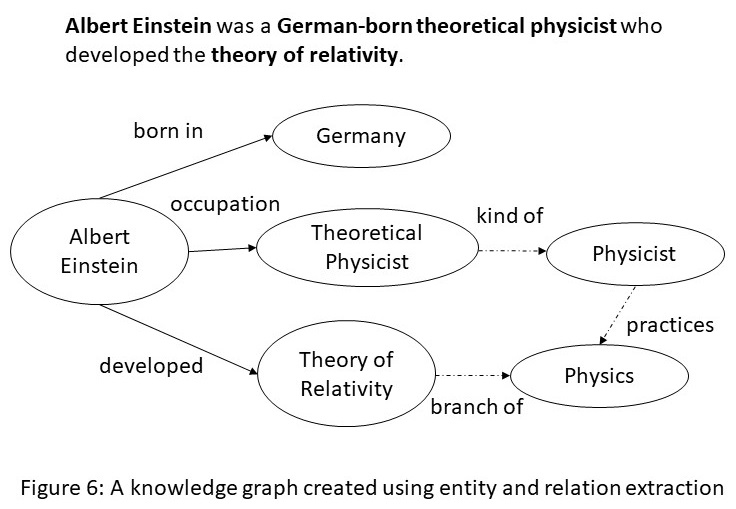
\includegraphics[width=1\linewidth]{figs/image2.jpg}
			\label{fig:writing-thesis}
		\end{figure}
	\end{frame}
	\begin{frame}{Đồ thị tri thức là đầu ra của Học Máy}
		\begin{figure}[H]
			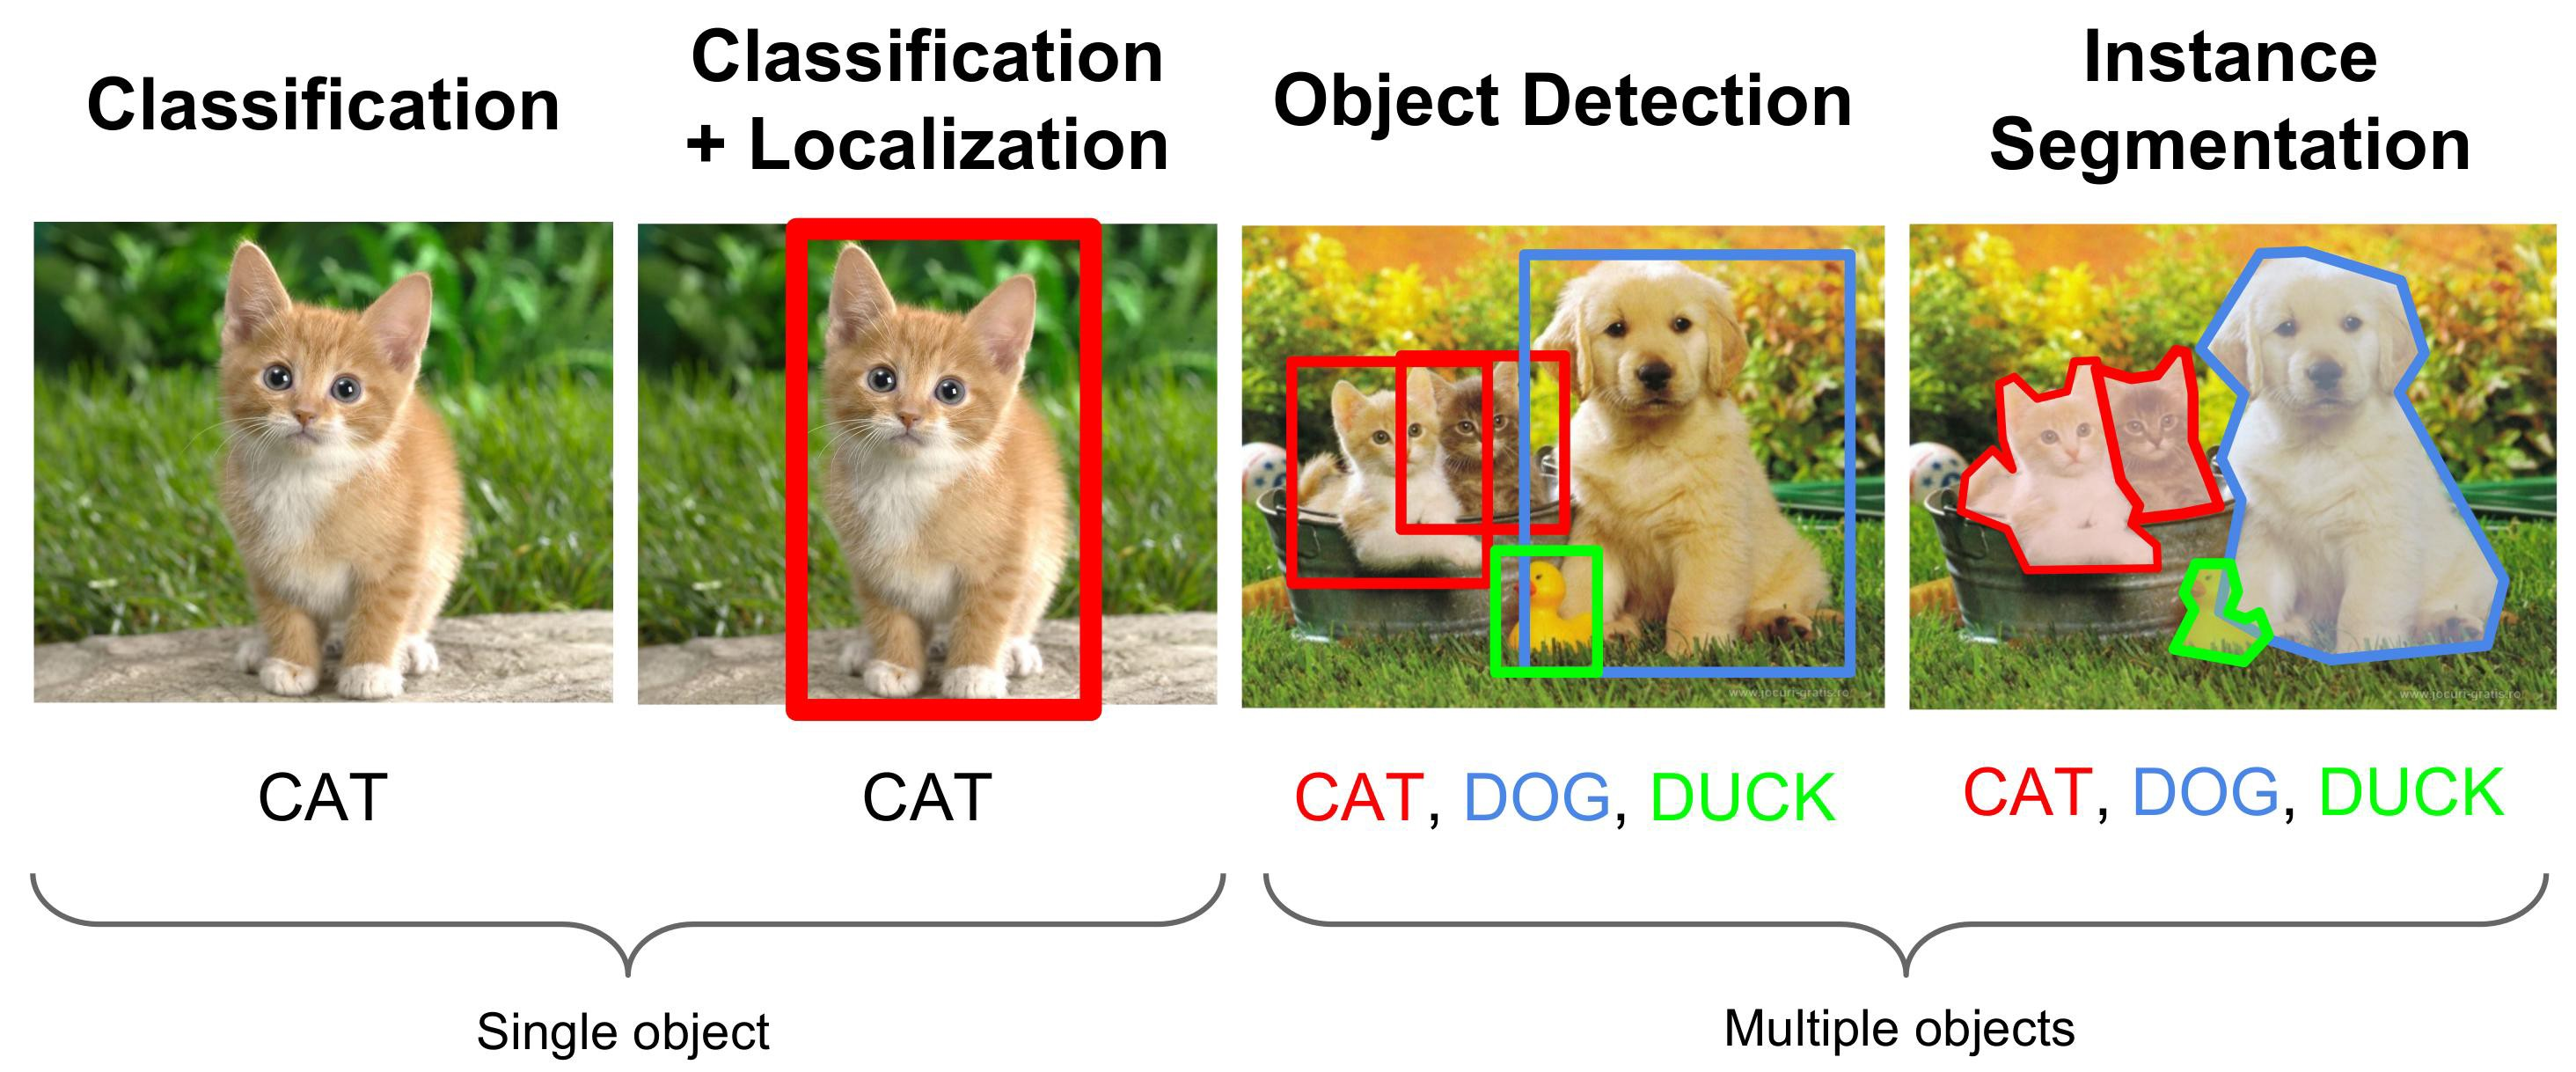
\includegraphics[width=0.5\linewidth]{figs/img.jpg}
			\label{fig:writing-thesis}
		\end{figure}
		\begin{figure}[H]
			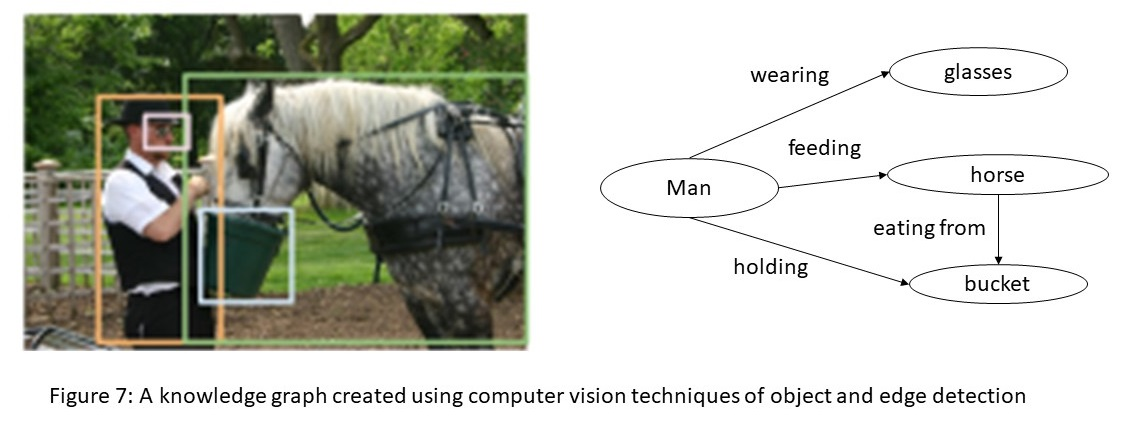
\includegraphics[width=1\linewidth]{figs/image6.jpg}
			\label{fig:writing-thesis}
		\end{figure}
	\end{frame}
	\begin{frame}{Đồ thị tri thức là đầu vào của Học Máy}
		\begin{figure}[H]
			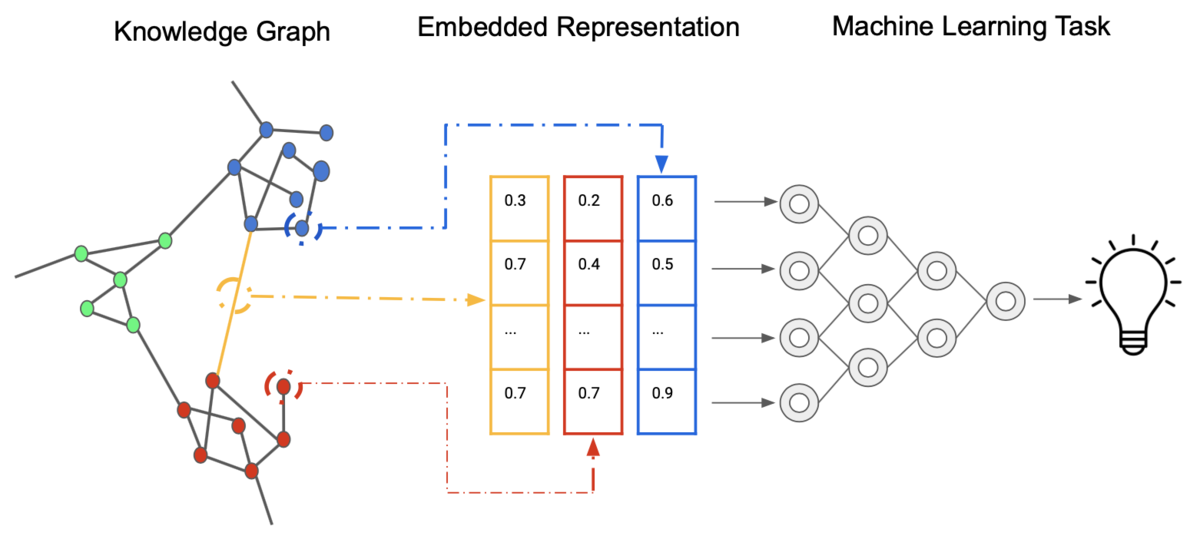
\includegraphics[width=1\linewidth]{figs/KnowledgeGraphEmbedding.png}
			\label{fig:writing-thesis}
		\end{figure}
	\end{frame}
	\section{Bài toán hoàn thiện đồ thị tri thức}
	\subsection{Động lực nghiên cứu khoa học}
	\begin{frame}{Động lực nghiên cứu khoa học}
		\begin{itemize}
			\item Hầu hết các đồ thị tri thức được xây dựng thủ công hoặc bán tự động
			\item Một lượng lớn thực thể và quan hệ tiềm ẩn chưa được khám phá
		\end{itemize}
	\begin{figure}[H]
		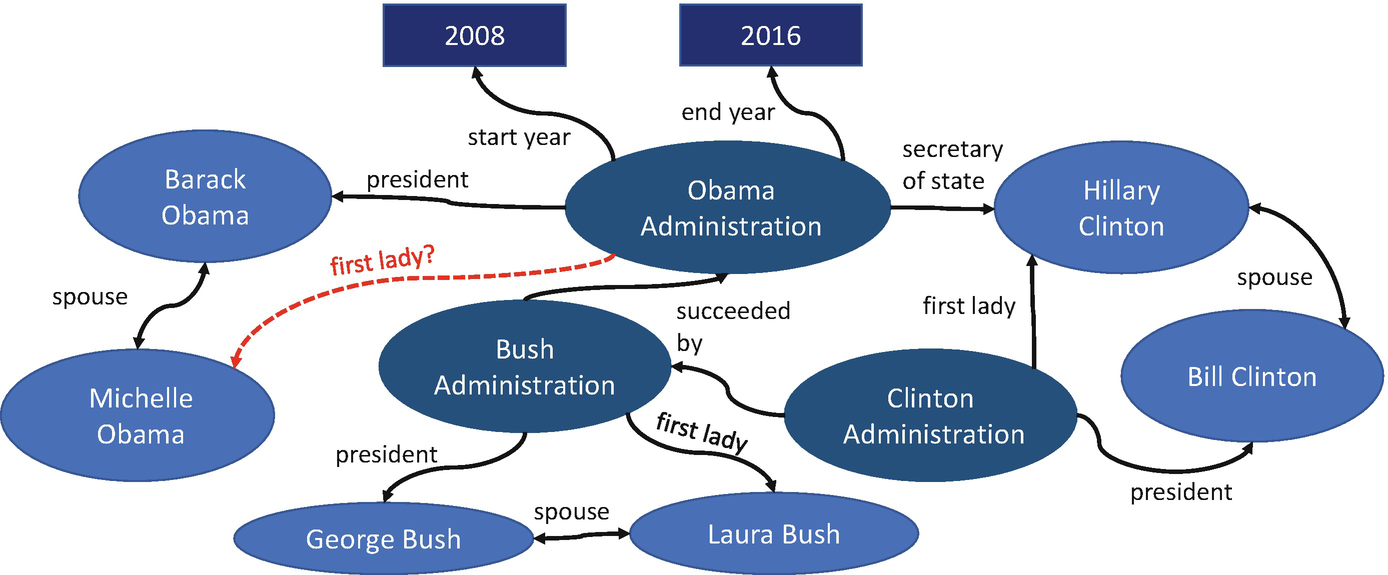
\includegraphics[width=1\linewidth]{figs/463227_1_En_4_Fig1_HTML.png}
		\label{fig:writing-thesis}
	\end{figure}
	\end{frame}
	\subsection{Phát biểu bài toán}
	\begin{frame}{Phát biểu bài toán}
		\begin{itemize}
			\item Đầu vào (Input): Đồ thị tri thức $\mathcal{G} = \{\mathcal{E}, \mathcal{R}, \mathcal{F}\}$, $\mathcal{F} = (h, r, t)$
			\item Đầu ra (Output): Ước lượng triển vọng của những thành phần bị thiếu trong bộ ba
		\end{itemize}
	\begin{figure}[H]
		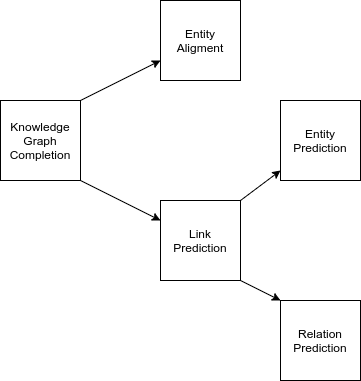
\includegraphics[width=0.5\linewidth]{figs/problem_divided.png}
		\label{fig:writing-thesis}
	\end{figure}
	\end{frame}
	\begin{frame}{Phát biểu bài toán}
		\textbf{Bài toán Entity Alignment}
		\begin{itemize}
			\item Đầu vào (Input): Đồ thị tri thức $\mathcal{G}_1 = \{\mathcal{E}_1, \mathcal{R}_1, \mathcal{F}_1\}$, $\mathcal{F}_1 = (h, r, t)$ và  $\mathcal{G}_2 = \{\mathcal{E}_2, \mathcal{R}_2, \mathcal{F}_2\}$, $\mathcal{F}_1 = (h, r, t)$
			\item Đầu ra (Output):$A = \{(e_1, e_2) \in \mathcal{E}_1 \times \mathcal{E}_2 \|\ e_1 \equiv e_2\}$
		\end{itemize}
		\textbf{Bài toán Link Prediction}
		\begin{itemize}
			\item Đầu vào (Input): Cho trước $(?, r, t)$ hoặc $(h, r, ?)$ hoặc $(h, ?, t)$
			\item Đầu ra (Output): Danh sách có xếp hạng của những thục thể/ quan hệ có triển vọng để thay thế "?"
		\end{itemize}
	\end{frame}
	\subsection{Phương pháp giải toán}
	\begin{frame}{Các phương pháp tiếp cận}
		\begin{figure}[H]
			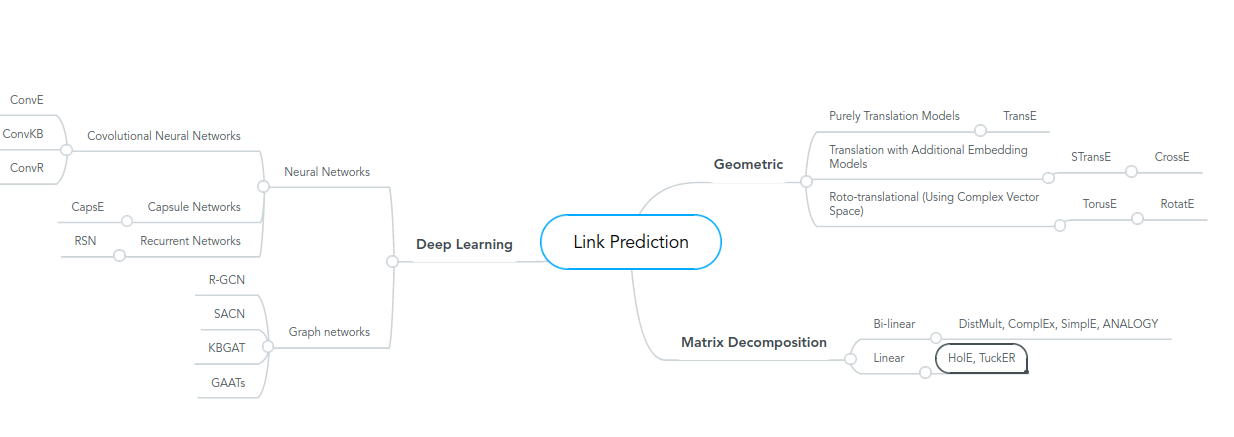
\includegraphics[width=1\linewidth]{figs/mindmap.png}
			\label{fig:writing-thesis}
		\end{figure}
	\end{frame}
	\begin{frame}{Các phương pháp tiếp cận: Hình học}
		\begin{figure}[H]
			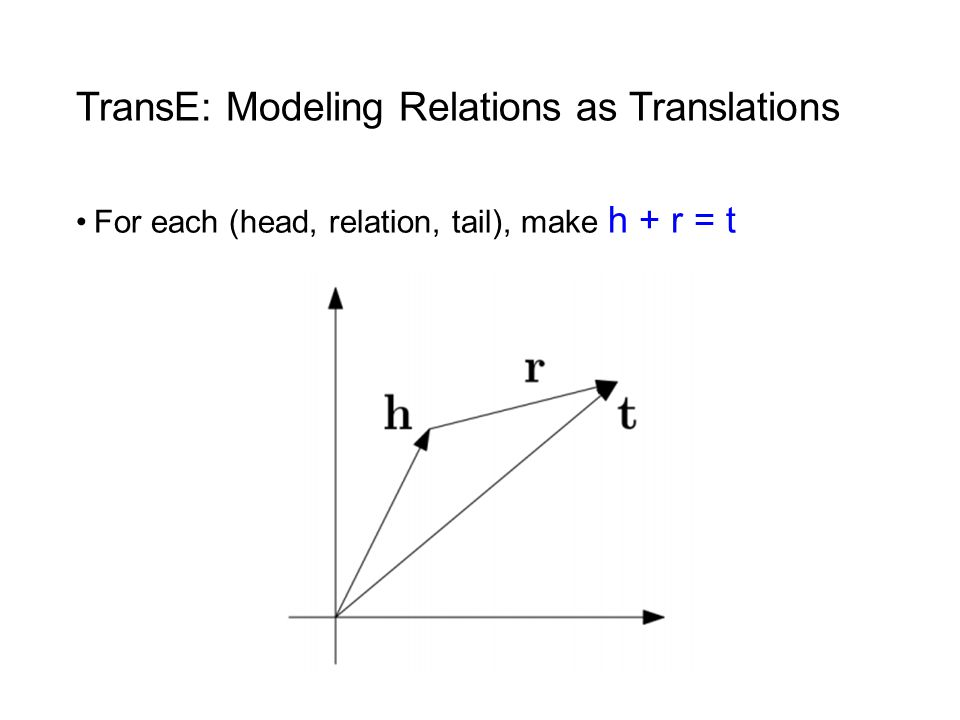
\includegraphics[width=1\linewidth]{figs/TransE.jpg}
			\label{fig:writing-thesis}
		\end{figure}
	\end{frame}
	\begin{frame}{Các phương pháp tiếp cận: Phân rã ma trận/ tensor}
		\begin{figure}[H]
			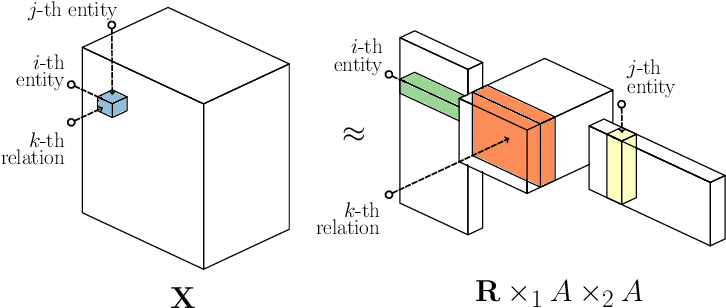
\includegraphics[width=1\linewidth]{figs/RESCAL.png}
			\caption{Mô hình RESCAL}
			\label{fig:writing-thesis}
		\end{figure}
	\end{frame}
	\begin{frame}{Các phương pháp tiếp cận: Neural Networks}
		\begin{figure}[H]
			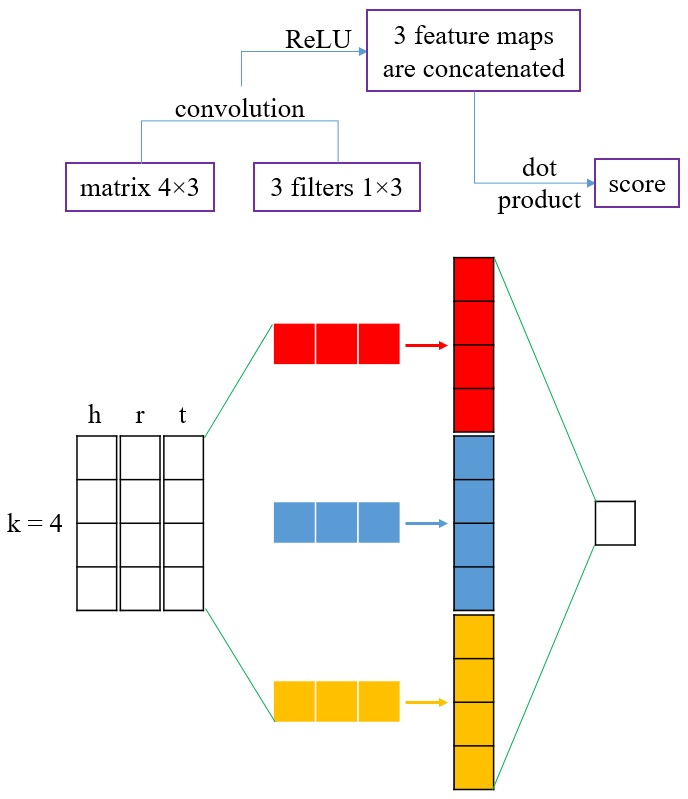
\includegraphics[width=0.5\linewidth]{figs/ConvKB.png}
			\caption{Mô hình ConvKB}
			\label{fig:writing-thesis}
		\end{figure}
	\end{frame}
	\begin{frame}{Các phương pháp tiếp cận: Graph Networks}
		\begin{figure}[H]
			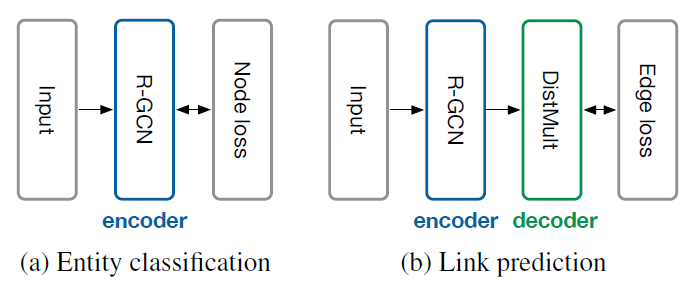
\includegraphics[width=1\linewidth]{figs/graph_nets_01.png}
			\label{fig:writing-thesis}
		\end{figure}
	\end{frame}
	\section{Tài liệu tham khảo}
	\begin{frame}{Tài liệu tham khảo}
		\nocite{*}
		\bibliography{references}\newpage\cleardoublepage
		\bibliographystyle{plain}
	\end{frame}
	\begin{frame}{Kết luận và Trả lời câu hỏi}
		Kết luận
		\begin{itemize}
			\item Giới thiệu chung về đồ thị tri thức
			\item Bài toán họàn thiện đồ thị tri thức
			\item Giới thiệu một số phương pháp cho bài toán dự đoán liên kết
		\end{itemize}
		Dự kiến chủ đề kế tiếp: Giới thiệu tổng quan Graph Neural Networks
		\begin{itemize}
			\item Cơ bản về mạng neural: Neuron, Back Propagation, Neural Network
			\item Vanilla Graph Neural Network, Graph Convolutional Networks
		\end{itemize}
		Cảm ơn các bạn đã theo dõi và lắng nghe!
		
		Mời các bạn đặt câu hỏi
	\end{frame}
\end{document}